\chapter{Results of Research and Conclusions}
\section{Evaluation of CNN Models}
\subsection{Radiography CNN Models}
\subsection{Chest X-Ray CNN Models}
\subsection{X-Ray Dataset Covid 19 CNN Models}
\section{Evaluation of GAN Models}
\subsection{Radiography GAN Models}
\subsubsection{Radiography DCGAN for COVID-19 Augmentation}
The radiography DCGAN for synthetically generated COVID-19 samples had mixed results.  Some of the images generated by the DCGAN came out looking very similar to the masks of patients lungs which were in the database.  I have included a side by side comparison in figure \ref{fig:Real COVID-19 Radiography Mask Example} and \ref{fig:Synthetically Generated COVID-19 Radiography Mask Example DCGAN} below
 \begin{figure}[H]
    \centering
    \begin{subfigure}{.5\textwidth}
    \centering
      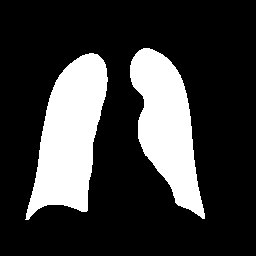
\includegraphics[width=.4\linewidth,keepaspectratio]{Images/Radiography_Real_Mask_COVID19_Example.png}
      \caption{Real COVID-19 Radiography Mask Example}
      \label{fig:Real COVID-19 Radiography Mask Example}
    \end{subfigure}%
    \begin{subfigure}{.5\textwidth}
    \centering
      
\includegraphics[width=.4\linewidth,keepaspectratio]{Images/Radiography_GAN_Mask_COVID19_Example.png}
      \caption{Generated COVID-19 Radiography Mask Example DCGAN}
      \label{fig:Synthetically Generated COVID-19 Radiography Mask Example DCGAN}
    \end{subfigure}%
\end{figure}
As is shown in the above images the synthetically generated COVID-19 mask looks relatively similar to the example taken from the dataset.  However not every single generated image came out as well as those that I have shown for demonstration purposes.  From reviewing the generated images it appears that a number of images bear no resemblance(or very little resemblance) to images within the data set.   
\\
From training a number of models there appears to be a need for pruning out bad images generated by the GAN and determining which images resemble X-Rays and Masks and which are "garbage" images which don't resemble data in our dataset.  This will require a lot of manual effort in determing which generated images are worth including in the augmented dataset and which are worth throwing away.
\subsection{Chest X-Ray GAN Models}
\subsection{X-Ray Dataset Covid 19 GAN Models}
\section{Possible Improvements}
\subsection{Larger Models}
\subsection{More Data Collection for GAN / CNN Training}
\subsection{More Computational Resources}
\section{Conclusion}